
\newcommand{\blkb}{\cellcolor[rgb]{0,0,0}\textcolor{white} 0 }
\newcommand{\bwn}{\cellcolor[rgb]{.26,.22,0}\textcolor{white} 9 }
\newcommand{\ora}{\cellcolor[rgb]{.44,.31,.15}8 }
\newcommand{\red}{\cellcolor[rgb]{.6,.4,.35}A }
\newcommand{\lgr}{\cellcolor[rgb]{.58,.58,.58}F }
\newcommand{\yel}{\cellcolor[rgb]{1.,.95,0.}7 }

\newcommand{\redb}{\cellcolor[rgb]{.6,.4,.35} 1 }

\chapter{Grafiek}
\label{cha:graphics}

Laten we nu eens plezier beleven aan grafiek! In dit deel van het boek willen wij de grafiekmodi van de MEGA65 bekijken door voorbeeldcode in machinetaal en BASIC stap voor stap te doorlopen, zodat u de verschillende mogelijkheden van de MEGA65 op het gebied van grafiek leert kennen. Allereerst is het belangrijk te weten dat de MEGA65 drie verschillende basisgrafiekmodi ondersteunt:

\begin{itemize}
	\item Bitmapgrafiek	\item Grafiek gebaseerd op tekensets	\item Bitplanes
\end{itemize}


\section*{Bitmapgrafiek}

In bitmapgrafiek wordt elke pixel van een afbeelding afzonderlijk opgeslagen. De manier waarop de pixels in het geheugen worden bewaard, verschilt van systeem tot systeem en hangt in de meeste gevallen af van de prestaties van de hardware. Als het geheugen onbeperkt zou zijn, zou de eenvoudigste manier om een pixel te onthouden zijn om zijn RGB-waarden in drie aparte bytes op te slaan. Voorbeeld: 0xFFFFFF voor wit zou betekenen dat er drie waarden opgeslagen moeten worden: \$FF, \$FF en \$FF. Eerlijk gezegd is dit te eenvoudig en niet echt efficiënt. Laten wij dus een andere manier bedenken. Waarom leggen wij niet een kleurentabel (of kleurenpalet) vast, slaan de RGB-waarden één keer op en verwijzen daarna alleen nog naar de kleur via de index ervan in de tabel? Dat bespaart ons veel geheugen! Stel dat wij een kleurrijke 8x8-bitmap maken, die op het scherm een ``A'' moet voorstellen. Kleurrijk wil hier zeggen dat wij hem in wat bruintinten willen hebben. De kleurentabel daarvoor kan er dan als volgt uitzien:

\begin{center}
\begin{tabular}{|l|l|}
\hline
	Index & Kleur \\
\hline
	\blkb & Zwart \\	\bwn & Bruin \\	\ora & Oranje \\	\red & Lichtrood \\	\lgr & Lichtgrijs \\	\yel & Geel \\
\hline
\end{tabular}
\end{center}

De kleurwaarden zijn overigens precies dezelfde als de kleurwaarden uit het standaard C64-kleurenpalet. Daarna ontwerpen we de ``A''. Elke pixel verwijst naar een waarde uit de bovenstaande kleurentabel.


\begin{center}
\begin{tabular}{|m{6pt}|m{6pt}m{6pt}m{6pt}m{6pt}m{6pt}m{5pt}m{6pt}m{6pt}|}
\hline
	& 7 & 6 & 5 & 4 & 3 & 2 & 1 & 0 \\
\hline
	0 & \blkb & \blkb & \blkb & \blkb & \blkb & \blkb & \blkb & \blkb \\	1 & \red & \lgr & \yel & \lgr & \red & \ora & \blkb & \blkb \\	2 & \lgr & \lgr & \blkb & \blkb & \ora & \red & \blkb & \blkb \\	3 & \yel & \yel & \blkb & \blkb & \ora & \red & \blkb & \blkb \\	4 & \yel & \lgr & \lgr & \red & \red & \red & \blkb & \blkb \\	5 & \lgr & \red & \blkb & \blkb & \ora & \red & \blkb & \blkb \\	6 & \red & \red & \blkb & \blkb & \red & \red & \blkb & \blkb \\	7 & \ora & \bwn & \blkb & \blkb & \ora & \red & \blkb & \blkb \\
\hline
\end{tabular}
\end{center}

Hoeveel geheugen gebruikt dit kleine afbeeldingetje eigenlijk?

Als we een eendimensionale array maken, krijgen we een array met 64 elementen, want onze afbeelding bestaat uit 8x8 pixels = 64 kleurwaarden die opgeslagen moeten worden. Vertaald naar het geheugen van de MEGA65 betekent dit dat we 64 bytes in het geheugen moeten bewaren. Een afbeelding die het volledige scherm vult, bestaat evenwel uit veel meer pixels. Op de C64 en natuurlijk ook op de MEGA65 zijn 320x200 pixels nodig om een afbeelding te maken die het hele scherm vult. Als we dat naar onze array doorrekenen, komen we uit op in totaal 64000 elementen. Omgerekend naar het geheugen van de MEGA65 zijn dat 64000 bytes, oftewel bijna 64 kilobyte aan gegevens! Als we daarbij ook nog bedenken dat de goede oude C64 slechts over 64K RAM beschikte, dan wordt de dramatiek duidelijk! Dat is simpelweg veel te veel gegevens! We hebben strategieën nodig om onze bitmapgegevens te beperken. Op de C64 waren er twee typen bitmapgrafieken, elk met zijn eigen mechanismen om het geheugengebruik tot een minimum te beperken.

\begin{itemize}
	\item Hires	\item Multicolour (MCM)
\end{itemize}


\subsection*{Hires}

Allereerst delen we een bitmap op in blokken van elk 8x8 pixels. Om de volledige resolutie van 320x200 pixels te bereiken, vormen 40 van zulke blokken naast elkaar één regel. Bouwen we vervolgens 25 van die regels op, dan komen we uit op een afbeelding die het volledige scherm vult.

\begin{adjustbox}{width=\textwidth,center}
\begin{footnotesize}
\begin{tabular}[h]{|C{10pt}|C{5pt}|C{5pt}|C{5pt}|C{5pt}|C{5pt}|C{5pt}|C{5pt}|C{5pt}|C{5pt}|C{5pt}|C{5pt}|C{5pt}|C{5pt}|C{5pt}|C{5pt}|C{5pt}|C{5pt}|C{5pt}|C{5pt}|C{5pt}|C{5pt}|C{5pt}|C{5pt}|C{5pt}|C{5pt}|C{5pt}|C{5pt}|C{5pt}|C{5pt}|C{5pt}|C{5pt}|C{5pt}|C{5pt}|C{5pt}|C{5pt}|C{5pt}|C{5pt}|C{5pt}|C{5pt}|C{5pt}|}
\hline
  &   &   &  &  &  &   &   &   &   & 1  & 1  & 1  & 1  & 1  & 1  & 1  & 1  & 1  & 1  & 2  & 2  & 2  & 2  & 2  & 2  & 2  & 2  & 2  & 2  & 3  & 3  & 3  & 3  & 3  & 3  & 3  & 3  & 3  & 3  & 4  \\  & 1 & 2 & 3& 4& 5& 6 & 7 & 8 & 9 &  0 & 1  &  2 &  3 &  4 &  5 &  6 &  7 &  8 &  9 &  0 &  1 &  2 &  3 &  4 &  5 &  6 &  7 &  8 &  9 &  0 &  1 &  2 &  3 &  4 &  5 &  6 &  7 &  8 &  9 &  0 \\
\hline
   1 & & & & & & & & & & & & & & & & & & & & & & & & & & & & & & & & & & & & & & & & \\\hline   2 & & & & & & & & & & & & & & & & & & & & & & & & & & & & & & & & & & & & & & & & \\\hline   3 & & & & & & & & & & & & & & & & & & & & & & & & & & & & & & & & & & & & & & & & \\\hline   4 & & & & & & & & & & & & & & & & & & & & & & & & & & & & & & & & & & & & & & & & \\\hline   5 & & & & & & & & & & & & & & & & & & & & & & & & & & & & & & & & & & & & & & & & \\\hline   6 & & & & & & & & & & & & & & & & & & & & & & & & & & & & & & & & & & & & & & & & \\\hline   7 & & & & & & & & & & & & & & & & & & & & & & & & & & & & & & & & & & & & & & & & \\\hline   8 & & & & & & & & & & & & & & & & & & & & & & & & & & & & & & & & & & & & & & & & \\\hline   9 & & & & & & & & & & & & & & & & & & & & & & & & & & & & & & & & & & & & & & & & \\\hline  10 & & & & & & & & & & & & & & & & & & & & & & & & & & & & & & & & & & & & & & & & \\\hline  11 & & & & & & & & & & & & & & & & & & & & & & & & & & & & & & & & & & & & & & & & \\\hline  12 & & & & & & & & & & & & & & & & & & & & & & & & & & & & & & & & & & & & & & & & \\\hline  13 & & & & & & & & & & & & & & & & & & & & & & & & & & & & & & & & & & & & & & & & \\\hline  14 & & & & & & & & & & & & & & & & & & & & & & & & & & & & & & & & & & & & & & & & \\\hline  15 & & & & & & & & & & & & & & & & & & & & & & & & & & & & & & & & & & & & & & & & \\\hline  16 & & & & & & & & & & & & & & & & & & & & & & & & & & & & & & & & & & & & & & & & \\\hline  17 & & & & & & & & & & & & & & & & & & & & & & & & & & & & & & & & & & & & & & & & \\\hline  18 & & & & & & & & & & & & & & & & & & & & & & & & & & & & & & & & & & & & & & & & \\\hline  19 & & & & & & & & & & & & & & & & & & & & & & & & & & & & & & & & & & & & & & & & \\\hline  20 & & & & & & & & & & & & & & & & & & & & & & & & & & & & & & & & & & & & & & & & \\\hline  21 & & & & & & & & & & & & & & & & & & & & & & & & & & & & & & & & & & & & & & & & \\\hline  22 & & & & & & & & & & & & & & & & & & & & & & & & & & & & & & & & & & & & & & & & \\\hline  23 & & & & & & & & & & & & & & & & & & & & & & & & & & & & & & & & & & & & & & & & \\\hline  24 & & & & & & & & & & & & & & & & & & & & & & & & & & & & & & & & & & & & & & & & \\\hline  25 & & & & & & & & & & & & & & & & & & & & & & & & & & & & & & & & & & & & & & & & \\\hline
\end{tabular}
\end{footnotesize}
\end{adjustbox}

De opdeling in blokken is zinvol, want daardoor kunnen wij de gegevens aanzienlijk verkleinen. Elke regel van een 8x8-blok bestaat uit 8 bits, dus waarom zouden wij de kleurindexen niet loslaten en simpelweg afspreken dat een gezette pixel een ``1'' in de regel voorstelt en een niet-gezette pixel overeenkomt met ``0''.

\begin{center}
\begin{tabular}{|C{12pt}|C{12pt}C{12pt}C{12pt}C{12pt}C{12pt}C{12pt}C{12pt}C{12pt}|R{24pt}|R{24pt}|}
\hline
	& 7 & 6 & 5& 4& 3&  2& 1& 0 & dec & hex \\
\hline
0 & \blkb & \blkb & \blkb & \blkb & \blkb & \blkb & \blkb & \blkb &   0 & 00 \\1 & \blkb & \redb & \redb & \redb & \redb & \blkb & \blkb & \blkb & 120 & 78 \\2 & \redb & \redb & \blkb & \blkb & \redb & \redb & \blkb & \blkb & 204 & CC \\3 & \redb & \redb & \blkb & \blkb & \redb & \redb & \blkb & \blkb & 204 & CC \\4 & \redb & \redb & \redb & \redb & \redb & \redb & \blkb & \blkb & 252 & FC \\5 & \redb & \redb & \blkb & \blkb & \redb & \redb & \blkb & \blkb & 204 & CC \\6 & \redb & \redb & \blkb & \blkb & \redb & \redb & \blkb & \blkb & 204 & CC \\7 & \redb & \redb & \blkb & \blkb & \redb & \redb & \blkb & \blkb & 204 & CC \\
\hline
\end{tabular}
\end{center}

Zoals hierboven te zien is, kunt u de bits van elke regel nu eenvoudig omrekenen naar de bijbehorende hexadecimale waarde en houdt u uiteindelijk 8 bytes aan gegevens over. Dit is de centrale gedachte achter hires-grafiek en met dit concept bespaart u veel geheugen. In dit voorbeeld zijn het 8 bytes, tegenover het vorige voorbeeld, waarin 64 bytes nodig waren om alle kleurverwijzingen te beheren. Rekenen we het eens door voor een afbeelding die het volledige scherm vult: we hebben 40x25 blokken, dat zijn er in totaal 1000. Elk blok is 8 bytes, dus dat levert ``slechts'' 8K op voor een afbeelding op volledig scherm.\\

Dit is een briljante oplossing, maar nu hebben wij een probleem: wij zijn de kleuren kwijt!\\

Als u naar de eerste afbeelding kijkt, ziet u dat die erg kleurrijk was. Hebben we die vele kleuren echter wel nodig? Dit is het tweede belangrijke concept in hires-bitmapgrafiek: minder kleuren betekent minder geheugen. De hires-modus beperkt u in feite tot \textbf{twee kleuren} per 8x8-pixelblok. Deze informatie wordt bewaard in het schermgeheugen (Screen-RAM) en niet, zoals u misschien zou aannemen, in het kleurengeheugen (Colour-RAM). Ook het idee erachter is opnieuw erg vernuftig: in het schermgeheugen kunt u waarden tussen \$00 en \$FF bewaren, terwijl het in het kleurengeheugen alleen zin heeft om waarden tussen \$0 en \$0F op te slaan, om één specifieke kleur uit het C64-kleurenpalet aan te duiden, dat uit 16 kleuren bestaat (\$0-\$F). Op de MEGA65 zijn zelfs nog meer kleuren mogelijk en u kunt de standaardkleuren aanpassen, maar dat wordt later uitgelegd.\\

Terug naar het schermgeheugen. Hier bewaart u \textbf{twee kleuren} voor elk 8x8-blok. Als u de byte splitst in zijn hoge en lage nibble, heeft u de mogelijkheid om er een achtergrond- en een voorgrondkleur in onder te brengen! De hexadecimale waarde \$0a bijvoorbeeld kunt u lezen als \$0 (hoge nibble) en \$a (lage nibble). Op die manier krijgen wij een zwarte achtergrond en lichtrood voor de pixels in het blok. Uiteindelijk betekent dit dat een hires-bitmap voor het volledige scherm niet 8 maar 9 kilobyte gebruikt: 8K voor de ruwe bitmapgegevens, zoals eerder genoemd, en nog eens 1K voor de kleuren in het schermgeheugen.\\

\subsection*{Eenvoudige hires-bitmaps programmeren}

Laten we gaan programmeren! We doen dat eerst in BASIC, voordat we overschakelen naar machinetaal. Om bitmapgrafieken op het scherm te brengen, moeten we de VIC-IV-chip configureren. De VIC moet een paar dingen weten voordat de chip de bitmapgegevens kan vinden en lezen. U moet het volgende doen:

\begin{itemize}
	\item Zorg dat u de VIC-registers heeft geactiveerd die u nodig heeft (denk eraan: de MEGA65 biedt verschillende versies van de VIC-chip)	\item Stel de resolutie in	\item Bepaal een locatie voor de bitmapgegevens	\item En schakel ten slotte de bitmapmodus in
\end{itemize}

Al deze instellingen kunt u in verschillende registers van uw MEGA65 configureren. Een overzicht van de bestaande registers van de grafische chip (dat is uiteraard de VIC) vindt u in \bookvref{cha:viciv}.

Uw MEGA65 bevat één grafische chip, de \textbf{VIC-IV}, die voortbouwt op zijn twee voorgangers en aan die voorgangers nieuwe functies in de vorm van extra registers toevoegt. Deze twee voorgangers zijn de \textbf{VIC-II}, zoals die in de oorspronkelijke Commodore 64 werd gebruikt, en de \textbf{VIC-III}, ook wel ``Bill'' genoemd, zoals die voor de Commodore 65 was gepland.

Het is belangrijk te begrijpen dat deze verschillende VIC-versies op elkaar voortbouwen; beschouw ze als modi die u aan of uit kunt zetten. VIC-III breidt de bestaande registers van de VIC-II uit, terwijl de VIC-IV u alle bestaande registers van VIC-II en VIC-III biedt en daarop voortbouwt door aan eerder ongebruikte registers nieuwe functionaliteit toe te voegen. Dat betekent dat in \bookvref{cha:viciv} niet alleen de registers van de VIC-IV belangrijk zijn om te kennen, maar ook die van VIC-II en VIC-III, afhankelijk van welke VIC-modus u wel of niet heeft geactiveerd. Houd hiermee rekening.

\textbf{Zorg dat u de VIC-registers heeft geactiveerd die u nodig heeft} - wat betekent dat? In grote lijnen gebruikt u het nieuwe register \$D02F hex of 53295 decimaal om tussen de VIC-modi te schakelen (d.w.z. om specifieke registers toe te voegen of te verwijderen). Voor het schakelen gebruikt u een zogeheten klopsequentie, door achtereenvolgens twee specifieke waarden te poken:

\begin{tabular}{|l|l|l|}
	\hline
	VIC & Eerste hex/dec & Tweede hex/dec \\
	\hline
	II  & \$00/0 & \$00/0\\	III & \$A5/165 & \$96/150\\	IV  & \$47/71 & \$53/83\\
	\hline
\end{tabular}

Terzijde: de twee waarden waarmee u de VIC-IV activeert, zijn de ASCII-tekens ``G'' en ``S''. Dat zijn de initialen van de maker van de VIC-IV: universitair hoofddocent Paul Gardner-Stephen. Een leuk paaseitje, nietwaar?

Het is belangrijk te begrijpen dat de computer, wanneer u uw MEGA65 inschakelt, in de C64-modus start en vervolgens zoekt naar een C65-compatibele ROM. Wordt een C64-cartridge gedetecteerd of drukt u de MEGA-toets in, dan blijft het systeem in de C64-modus. In dat geval heeft u alleen de C64-registers tot uw beschikking. Vindt het systeem een C65-ROM, dan activeert het de beschikbare registers. Bij de MEGA65-ROM betekent dit dat u alle VIC-registers (II, III en IV) kunt benaderen. Geeft u het GO64-commando, dan beperkt het systeem u tot de VIC-II-registers - maar denk eraan - door de klopsequentie zoals hierboven beschreven uit te voeren, kunt u die registers weer toevoegen! Het maakt dus niet uit in welke ``modus'' u zich bevindt. Alle mogelijkheden zijn overal beschikbaar. De MEGA65 is werkelijk een flexibele machine!


In dit hoofdstuk gaan we ervan uit dat u in de C65-modus werkt en daarbij de standaard-ROM van de MEGA65 met BASIC65 gebruikt.


De volgende stap is het \textbf{instellen van de resolutie}. Volgens de registers in \bookvref{cha:viciv} kunt u dat doen met \$D031 hex, of 53297 decimaal. Dit register is afkomstig van VIC-III. De C65 beschikt over een beeldscherm met 80 kolommen, de C64 had er slechts 40. Om 80 kolommen te realiseren, moet de grafische chip met hogere resoluties overweg kunnen. Wanneer u de computer inschakelt, werkt u in de 80-kolomsmodus met 25 regels, hetgeen neerkomt op een resolutie van 640x200. Om klassieke bitmaps te tonen, moet u terug naar 320x200 (dat zijn de 40 kolommen en 25 regels, zoals al in de eerdere tabel te zien was). De C64 kon 640x200 niet weergeven, dus had de VIC-II geen register nodig om dat te regelen. De C65 beheerst daarentegen beide, zodat u met \$D031 ertussen kunt schakelen. Manipuleert u het register bitgewijs, dan kunt u nog meer instellen: de resolutie (databit 7, H640), de C65-fastmodus (databit 6, FAST) of het in- en uitschakelen van de nieuwe bitplane-modus als alternatief voor klassieke bitmap- of tekengebaseerde grafiek (databit 4, BPM). Sommige registers zijn wel gepland, maar nooit geïmplementeerd. Bijvoorbeeld een H1280-modus op databit 2, welke de C65 in staat moest stellen op te schalen naar 1280x200 of 1280x400. Zie \bookvref{cha:viciv} voor alle fijne details.

De volgende vraag is: hoe kunnen we specifieke bits in een register aansturen? Schakel uw computer in en typ het volgende commando in

\begin{screencode}
PRINT PEEK($D031)
 224
\end{screencode}

U krijgt dan een decimale waarde terug, zoals 224. De decimale waarde helpt u niet verder: u moet het getal omzetten naar zijn binaire voorstelling.

\begin{tabular}{|l|l|l|l|l|l|l|l|l|}
	\hline
	Bit 7 & Bit 6 & Bit 5 & Bit 4 & Bit 3 & Bit 2 & Bit 1 & Bit 0 & Decimale waarde \\	H640 & FAST & ATTR & BPM & V400 & H1280 & MONO & INT & ~ \\
	\hline
    1 & 1 & 1 & 0 & 0 & 0 & 0 & 0 & 224 \\    0 & 1 & 1 & 0 & 0 & 0 & 0 & 0 & 96 \\
	\hline
\end{tabular}

De eerste rij in de tabel toont het binaire getal voor decimaal 224; dit zou het geval moeten zijn wanneer u uw MEGA65 inschakelt. Databit 7, de H640-modus, is zoals verwacht geactiveerd. In de tweede rij ziet u de waarde die u moet gebruiken wanneer u wilt terugschakelen naar 320x200: databit 7 wordt op 0 gezet, zodat de H640-modus is uitgeschakeld.

\begin{screencode}
POKE $D031,96
\end{screencode}

Wacht echter even: de waarde rechtstreeks poken is niet altijd de juiste aanpak. Als u precies weet wat u doet - of beter: welke toestand elke bit van het register moet hebben - kunt u op deze manier verdergaan. Het wegschrijven van de waarde 96 betekent dat u alle databits in één keer instelt. Dat is niet altijd wat we willen. In sommige gevallen willen we slechts één specifieke bit manipuleren, bijvoorbeeld databit 7 voor de resolutie, terwijl de overige bits in hun bestaande toestand blijven. Dat bereikt u met logische bewerkingen, met behulp van de AND- of OR-operator.

\begin{tabular}{ ccc }
	~ & ~ & ~ \\
	% first table (AND)
	\begin{tabular}{ |c|c| }
		\hline
		Bewerking & Resultaat \\
		\hline
		0 AND 0 & 0  \\		1 AND 0 & 0  \\		0 AND 1 & 0  \\		1 AND 1 & 1  \\
		\hline
	\end{tabular} &
    % some space between the two tables
	\begin{tabular}{c}
	    \hspace{1cm} \\
	\end{tabular}
	% second table (OR)
	\begin{tabular}{ |c|c| }
   	    \hline
        Bewerking & Resultaat \\
		\hline
		0 OR 0 & 0  \\		1 OR 0 & 1  \\		0 OR 1 & 1  \\		1 OR 1 & 1  \\
		\hline
	\end{tabular} \\
\end{tabular}

De logische tabellen hierboven zijn belangrijk, omdat zij laten zien hoe de bits worden gewijzigd als u er een operator op toepast. Als u nadenkt over het idee van logische bewerkingen in het voorbeeld dat volgt, ziet u dat u AND kunt gebruiken om een specifieke bit op nul te zetten (te wissen, via een masker), en OR om de bit op 1 te zetten. Eerlijk gezegd is deze methode niet alleen bruikbaar om één enkele bit in te stellen, maar ook om een willekeurig aantal bits te wijzigen; om het eenvoudig te houden wijzigen we er slechts één. Terug naar de ``slechte'' poke van 96 die we hierboven zagen: die kunt u beter als volgt schrijven:

\begin{screencode}
  POKE $D031, PEEK($D031) AND 127 :REM RESET BIT 7 (d.w.z. zet het op nul)
  POKE $D031, PEEK($D031) OR 128  :REM ZET BIT 7 (d.w.z. zet het op één)
\end{screencode}

Om deze bewerkingen te begrijpen, moet u opnieuw elk decimaal getal omzetten naar zijn binaire vorm. Daarna passen we de AND / OR-bewerkingen bit voor bit toe, volgens de regels uit de voorgaande logische tabellen.
\begin{tabular}{ ccc }
	~ & ~ & ~ \\
	\begin{tabular}{|l|l|l|}
		\hline
		~ &  Binair & Decimaal\\
		\hline
		~ & 11100000 & 224\\		AND & 01111111 & 127\\
		\hline
		Resultaat & 01100000 & 96\\
		\hline
	\end{tabular} &
	% some space between the two tables
	\begin{tabular}{c}
		\hspace{1cm} \\
	\end{tabular}
	\begin{tabular}{|l|l|l|}
		\hline
		~ &  Binair & Decimaal\\
		\hline
		~ & 01100000 & 96\\		OR & 10000000 & 128\\
		\hline
		Resultaat & 11100000 & 224\\
		\hline
	\end{tabular} \\
\end{tabular}

Dit kunt u overigens testen met enkele eenvoudige PRINT-commando's:

\begin{screencode}
PRINT 224 AND 127
  96

PRINT 96 OR 128
  224
\end{screencode}

Gewapend met deze kennis kunnen we de VIC nu zodanig configureren dat deze bitmapgrafiek weergeeft. Daartoe moeten we een aantal registers fijnafstellen, maar voordat we daarmee kunnen beginnen, is het nodig om iets meer te begrijpen van de grafische chip, hoe deze is opgebouwd en vooral hoe hij het geheugen benadert.

\underline{Kanttekening}:

Een alternatieve aanpak, beschikbaar in BASIC 65 voor het zetten/wissen van bits, is het gebruik van de nieuwe {\bf SETBIT}- en {\bf CLRBIT}-commando's. Voor wie in assembleertaal programmeert, zijn bovendien de nieuwe instructies {\bf SMBx} (zet bit x) en {\bf RMBx} (wis bit x) beschikbaar.

\subsection*{De organisatie van de VIC-IV en de basis van geheugentoegang}

In tegenstelling tot de CPU van uw MEGA65, welke in één keer 64KB kan adresseren, kan de VIC dat helaas niet. Hij kan slechts 16KB overzien, dus u moet precies definiëren welke 16KB hij mag zien. Hiertoe wordt de 64KB van Bank 0 (dit is de geheugenbank waarin de VIC huist en zijn gegevens vandaan haalt) verdeeld in blokken van elk 16KB. Deze 16KB-blokken worden ``videobanken'' of ``VIC-banken'' genoemd.

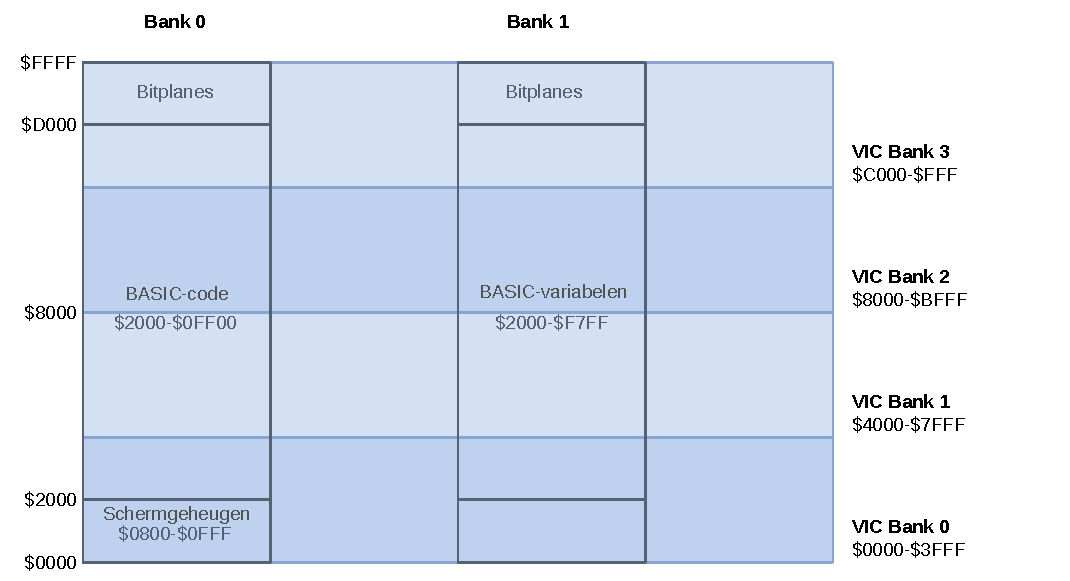
\includegraphics[width=\linewidth]{dutch/images/graphics/vic-banks.pdf}

Los van de VIC is het geheugenbeheer van de Commodore 65 of MEGA65 iets complexer dan dat van het vorige model. Dat komt doordat er in de machine meer geheugen beschikbaar is: bij de Commodore 65 waren 128KB gepland (mogelijk uit te breiden tot 1MB), terwijl de MEGA65 wordt geleverd met 384KB chip-RAM + 8MB zolder-RAM (mogelijk uit te breiden tot 256MB). Zoals eerder vermeld, kan de processor niet het hele geheugenbereik adresseren. Er is slechts 64KB zichtbaar. Om die reden is het geheugen verdeeld in blokken van elk 64KB en deze blokken worden ``banken'' genoemd.

Het systeem kan tot 16 banken hebben en bepaalde banken hebben daarnaast ook specifieke taken. Bank 0 en 1 zijn RAM, wat betekent dat u er zowel kunt lezen als schrijven, terwijl bank 2 en 3 ROM zijn en niet zo eenvoudig te overschrijven.

Bank 0 (gezien vanuit het besturingssysteem BASIC 65 dat start wanneer u de computer inschakelt) heet de systeembank. Deze bevat onder meer de volgende gebieden:

\begin{itemize}
  \item Het schermgeheugen, welke het geheugenbereik \$0800-\$2000 beslaat (standaard)  \item In het geheugen gemapte VIC-registers (indien deze zijn ingemapt, wat standaard het geval is)
\end{itemize}

Overigens staat de implementatie van BASIC65 zelf in ROM (bank 3), terwijl het BASIC van de C64 eveneens in ROM staat (bank 2).

Wilt u meer weten over geheugenbeheer in het algemeen, kijk dan bij \bookvref{cha:memory-map}. In BASIC is de situatie helaas nog complexer. Direct na het inschakelen van de computer bevindt u zich in Bank 128, een speciale bank met een speciale geheugenconfiguratie. U kunt het commando BANK gebruiken om tussen banken te wisselen. Een probleem daarbij is dat u gemakkelijk het overzicht verliest over wat er in welke bank staat of in welke bank u op dat moment werkt. Het is eigenlijk iets eenvoudiger wanneer u in machinetaal werkt. Voor meer informatie over het BANK-commando en over banken in het algemeen raadpleegt u \bookvref{BASIC 65 Commands!BANK}. Houd er rekening mee dat u eerst iets over banken moet weten voordat u op veilige wijze PEEK, POKE of SYS kunt gebruiken. Anders vraagt u zich misschien af waarom uw programma zich niet zo gedraagt als u verwachtte. Wij komen hier later op terug. Terug naar de grafiek.

Laten we beginnen met het schrijven van een eenvoudig BASIC-programmaatje om hires-bitmapgrafiek weer te geven. Indien u dit hoofdstuk tot op dit punt zorgvuldig heeft gevolgd, zult u geen moeite hebben met het begrijpen van de volgende coderegels:

\begin{screencode}
10 POKE $D020,0 : POKE $D021,0          :REM MAAK SCHERM ZWART
20 POKE $D031, PEEK($D031) AND 127      :REM STEL RESOLUTIE IN
30 POKE $DD02, 3                        :REM MAAK VIRTUALE CIA-2 LEES- EN SCHRIJFBAAR
40 POKE $$DD00, PEEK($DD00) AND 252 OR 2:REM KIES VIDEOBANK 1
\end{screencode}

Zoals u op de afbeelding op de vorige bladzijde heeft gezien, verdeelt de VIC-chip het geheugen in 4 videobanken van elk 16KB. Het is belangrijk te begrijpen dat u geen register van de VIC gebruikt om de videobank binnen (geheugen-)bank 0 te definiëren; in plaats daarvan gebruikt u de databits 0 en 1 van \$DD00 of decimaal 56576. Dit was ooit een register van de CIA-2-chip in de Commodore 64, maar in uw MEGA65 is het geïmplementeerd als virtueel register. De ``voorbereiding'' die nodig is om de videobank in te stellen, gebeurt in regel 30, terwijl in de daaropvolgende regel de videobank zelf wordt ingesteld. Overigens geldt: als u de decimale waarde 3 (regel 30) omzet naar binair formaat, is dat 00000011 en dat bewijst dat de databits 0 en 1 op 1 staan, zodat lezen en schrijven is geactiveerd.

{\small
\begin{tabular}{|c|c|l|l|}
	\hline
	Bits & VIC-bank & Geheugengebied & BASIC \\
	\hline
	 \textbf{00} & 3 & \$C000-\$FFFF & ... AND 252 OR 0 :REM AND 11111100 OR 000000\textbf{00} \\
	 \textbf{01} & 2 & \$8000-\$BFFF & ... AND 252 OR 1 :REM AND 11111100 OR 000000\textbf{01} \\
	 \textbf{10} & 1 & \$4000-\$7FFF & ... AND 252 OR 2 :REM AND 11111100 OR 000000\textbf{10} \\
	 \textbf{11} & 0 & \$0000-\$3FFF & ... AND 252 OR 3 :REM AND 11111100 OR 000000\textbf{11} \\
	\hline
\end{tabular}
}

De tabel toont welke bits moeten worden ingesteld om een videobank te selecteren.
